 \documentclass[column,amsmath,amssymb,floatfix]{revtex4}

% ---- Pacotes para formatação de texto e símbolos matemáticos ----
\usepackage{amsmath}
\usepackage{amssymb}
\usepackage{amsfonts}

% ---- Pacotes para gráficos e tabelas ----
\usepackage{graphicx}
\usepackage{dcolumn}
\usepackage{float}
\usepackage{graphicx}     % Para imagens
\usepackage{subcaption}   % Para subfiguras

% ---- Pacotes para formatação e personalização de cores e fontes ----
\usepackage{xcolor}
\usepackage{color}
\usepackage{bm}
\usepackage{titlesec}
\usepackage{enumitem}

% ---- Pacotes para código fonte ----
\usepackage{listings}
\usepackage{verbatim}

\lstdefinestyle{customc}{
  belowcaptionskip=1\baselineskip,
  breaklines=true,
  frame=none,
  xleftmargin=\parindent,
  language=python,
  showstringspaces=false,
  basicstyle=\footnotesize\ttfamily,
  keywordstyle=\bfseries\color{green!40!black},
  commentstyle=\itshape\color{purple!40!black},
  identifierstyle=\color{blue},
  stringstyle=\color{orange},
}

\lstdefinestyle{customasm}{
  belowcaptionskip=1\baselineskip,
  frame=trBL,
  xleftmargin=\parindent,
  language=[x86masm]Assembler,
  basicstyle=\footnotesize\ttfamily,
  commentstyle=\itshape\color{purple!40!black},
}

\lstset{
 escapechar=@,
 style=customc,
 inputencoding=utf8, 
 extendedchars=true,
 literate={á}{{\'{a}}}1 {ã}{{\~{a}}}1 {é}{{\'{e}}}1 {ê}{{\^{e}}}1 {í}{{\'{i}}}1 
          {ó}{{\'{o}}}1 {õ}{{\~{o}}}1 {ú}{{\'{u}}}1 {ç}{{\c{c}}}1,
 keepspaces=true,
 columns=flexible,
 basicstyle=\ttfamily
}
% ---- Pacotes de idioma e codificação ----
\usepackage[brazilian]{babel}
\usepackage[utf8]{inputenc}
\usepackage[T1]{fontenc}

% ---- Pacote para criação de links e hiperlinks ----
\usepackage{hyperref}

% ---- Definição de comandos personalizados ----
\newcommand{\PAR}[1]{\left({[#1]}\right)}

% ---- Ajustes de espaçamento para títulos ----
\titlespacing\section{0pt}{12pt plus 4pt minus 2pt}{8pt plus 2pt minus 2pt}
\titlespacing\subsection{0pt}{12pt plus 4pt minus 2pt}{8pt plus 2pt minus 2pt}
\titlespacing\subsubsection{0pt}{12pt plus 4pt minus 2pt}{0pt plus 2pt minus 2pt}

\begin{document}

\title{Relatório do EPREC - de Método Numéricos em Equações Diferenciais II}

\author{Lucas Amaral Taylor, NUSP: 13865062, graduação em Bacharelado em Matemática Aplicada e Computacional,  IME-USP}

\begin{abstract}
	\baselineskip 11pt
	Neste trabalho, aplicaremos o Método de Diferenças Finitas (MDF) para resolução numérica de equações de onda unidimensional utilizando conceitos apresentados em aula, com ênfase da utilização de derivada temporal de ordem dois.
\end{abstract}

\maketitle

\section{Introdução} 
No presente relatório, vamos estudar métodos numéricos aplicados em \textit{Python} para resolução da \textit{equação da velocidade da onda} dada por:
\begin{equation}
	u_{tt} = c^2 u_{xx}, \quad c>0.
	\label{eq:equacao-da-onda}
\end{equation}
em três problemas distintos. Em cada um deles, são fornecidas condições iniciais:
\begin{equation}
	u(x,0) = \Phi(x) \quad \text{ e } \quad u_t(x, 0) = \Psi(x)
	\label{eq:condicao-inicial-onda}
\end{equation}

Para a resolução, utilizaremos o esquema de diferenças finitas dado por:
\begin{align}
	U_m^{n+1} & = c^2\lambda^2(U_{m-1}^n + U_{m+1}^n) + 2(1-c^2\lambda^2)U_m^n - U_m^{n-1} \label{eq:edf-principal}                  \\
	U_m^0     & = \Phi(x_m) \label{eq:edf-inicial}                                                                                   \\
	U_m^1     & = \frac{c^2\lambda^2}{2}(\Phi_{m-1} + \Phi_{m+1}) + (1-c^2\lambda^2)\Phi_m + \tau\Psi_m \label{eq:edf-passo-inicial} 
\end{align}

As condições de fronteira consideradas são:
\begin{enumerate}[label=\roman*.]
	\item Dirichlet: $u(a,t) = \alpha(t)$ ou $u(b,t) = \beta(t)$
	\item Neumann: $u_x(a,t) = \phi(t)$ ou $u_x(b,t) = \psi(t)$
	\item Combinação das anteriores
\end{enumerate}

Utilizamos as seguintes aproximações para cada condição de fronteira:
\begin{enumerate}[label=\roman*.]
	\item Para Dirichlet:
	      \begin{align}
	      	\text{Se } u(a,t) & = \alpha(t): U_0^{n+1} = \alpha(t_{n+1}) \label{eq:dirichlet-a} \\
	      	\text{Se } u(b,t) & = \beta(t): U_M^{n+1} = \beta(t_{n+1}) \label{eq:dirichlet-b}   
	      \end{align}
	\item Para Neumann de ordem 1:
	      \begin{align}
	      	\text{Se } u_x(a,t) & = \phi(t): U_0^{n+1} = U_1^{n+1} - h\phi(t_{n+1}) \label{eq:neumman-1-a}     \\
	      	\text{Se } u_x(b,t) & = \psi(t): U_M^{n+1} = U_{M-1}^{n+1} + h\psi(t_{n+1}) \label{eq:neumman-1-b} 
	      \end{align}
	      	      
	\item Para Neumann de ordem 2:
	      \begin{align}
	      	\text{Se } u_x(a,t) & = \phi(t): U_0^{n+1} = \frac{4U_1^{n+1} - U_2^{n+1} - 2h\phi(t_{n+1})}{3}\label{eq:neumman-2-a}         \\
	      	\text{Se } u_x(b,t) & = \psi(t): U_M^{n+1} = \frac{4U_{M-1}^{n+1} - U_{M-2}^{n+1} + 2h\psi(t_{n+1})}{3}\label{eq:neumman-2-b} 
	      \end{align}    
\end{enumerate}

onde:
\begin{itemize}
	\item $u(x,t)$ é a solução exata no ponto $x$ e no instante $t$
	\item $U_m^n$ é a aproximação numérica de $u(x_m,t_n)$
	\item $c$ é a velocidade da onda
	\item $h$ é o espaçamento da malha espacial
	\item $\tau$ é o espaçamento da malha temporal
	\item $\lambda = \tau/h$ é a razão entre os espaçamentos
	\item $M$ é o número de pontos da malha espacial
	\item $x_m = a + mh$ são os pontos da malha espacial
	\item $t_n = n\tau$ são os pontos da malha temporal
	\item $\Phi(x)$ é a condição inicial de posição
	\item $\Psi(x)$ é a condição inicial de velocidade
\end{itemize}

\section{Descrição da parte teórica do trabalho}

\section{Implementação e explicação da resolução da tarefa}

A respeito da implementação da tarefa, temos que foi utilizado o ambiente \textit{Python} e as bibliotecas \texttt{matplotlib.pyplot} e \texttt{numpy}. Por questão de simplicidade, o programa foi desenvolvido em um único arquivo, \texttt{main.py}. O programa \texttt{main.py} é constituído por uma função principal, a função \texttt{main()} e outras cinco funções.

No que diz respeito à função \texttt{main()}, trata-se de um controle de fluxo para o usuário selecionar o exemplo trabalhado. No que diz respeito às outras, temos duas funções principais: \texttt{resolve\_eq\_onda()} e a função \texttt{aplica\_cond\_contorno()}, e três funções dedicadas a cada exemplo proposto pelo enunciado: \texttt{exemplo01()}, \texttt{exemplo02()} e \texttt{exemplo03()}. No presente relatório, vamos realizar uma análise mais profunda nas duas primeiras funções citadas e pontuar as particularidades das funções dedicadas à cada exemplo.



\subsection{Função \texttt{resolve\_eq\_onda()}}

A função \texttt{resolve\_eq\_onda()} é dada por:

\begin{lstlisting}
def resolve_eq_onda(a, b, T, h, lambda_val, c=1.0, phi=None, psi=None,
                    cont_esq=None, cont_dir=None,
                    tipo_cont_esq='dirichlet',
                    tipo_cont_dir='dirichlet',
                    ordem_neumann=2):
    """Resolve a equação da onda usando diferenças finitas."""
    M = int((b - a) / h)  # número de intervalos espaciais
    tau = lambda_val * h  # passo temporal
    N = int(T / tau)  # número de passos temporais

    # Pontos da malha
    x = np.linspace(a, b, M + 1)
    t = np.linspace(0, T, N + 1)
    U = np.zeros((N + 1, M + 1))

    # Condição inicial de posição
    if phi is not None:
        U[0, :] = phi(x)

    # Primeiro passo temporal usando velocidade inicial
    if psi is not None:
        U[1, 1:-1] = (c ** 2 * lambda_val ** 2 / 2) * (U[0, :-2] + U[0, 2:]) + \
                     (1 - c ** 2 * lambda_val ** 2) * U[0, 1:-1] + \
                     tau * psi(x[1:-1])

        # Aplica condições de fronteira no primeiro passo
        U[1, 0] = aplica_cond_contorno(U, t, 1, 0, cont_esq, tipo_cont_esq, h, ordem_neumann)
        U[1, -1] = aplica_cond_contorno(U, t, 1, M, cont_dir, tipo_cont_dir, h, ordem_neumann)

    # Loop principal no tempo
    for n in range(1, N):
        # Atualiza pontos interiores
        U[n + 1, 1:-1] = c ** 2 * lambda_val ** 2 * (U[n, :-2] + U[n, 2:]) + \
                         2 * (1 - c ** 2 * lambda_val ** 2) * U[n, 1:-1] - \
                         U[n - 1, 1:-1]

        # Aplica condições de contorno
        U[n + 1, 0] = aplica_cond_contorno(U, t, n + 1, 0, cont_esq, tipo_cont_esq, h, ordem_neumann)
        U[n + 1, -1] = aplica_cond_contorno(U, t, n + 1, M, cont_dir, tipo_cont_dir, h, ordem_neumann)

    return U, x, t
\end{lstlisting}
A função \texttt{resolve\_eq\_onda()} recebe os seguintes parâmetros:
\begin{itemize}
	\item \texttt{a, b}: Limites do intervalo espacial $[a,b]$
	\item \texttt{T}: Tempo final da simulação
	\item \texttt{h}: Passo espacial (discretização em $x$)
	\item \texttt{lambda\_val}: Razão $\tau/h$, onde $\tau$ é o passo temporal 
	\item \texttt{c}: Velocidade da onda (padrão = 1.0)
	\item \texttt{phi}: Função para condição inicial de posição $u(x,0)$
	\item \texttt{psi}: Função para condição inicial de velocidade $u_t(x,0)$
	\item \texttt{cont\_esq}: Função para condição de contorno em $x=a$
	\item \texttt{cont\_dir}: Função para condição de contorno em $x=b$
	\item \texttt{tipo\_cont\_esq}: Tipo da condição de contorno em $x=a$ (Dirichlet ou Neumann)
	\item \texttt{tipo\_cont\_dir}: Tipo da condição de contorno em $x=b$ (Dirichlet ou Neumann)
	\item \texttt{ordem\_neumann}: Ordem de aproximação para condições de Neumann (1 ou 2)
\end{itemize}

Nela, definidas as variáveis \texttt{M}, \texttt{tau} e \texttt{N}, estas relacionadas com a equação de diferenças finitas; as variáveis \texttt{x}, \texttt{t} e \texttt{u}, associadas com a malha de pontos. Após a definição de variáveis, o programa começa o tratamento com a condição inicial alinhado com as equações \eqref{eq:condicao-inicial-onda} e \eqref{eq:edf-inicial}. Por fim, são definidos os pontos interiores em dois laços. O primeiro é responsável pelo cálculo do primeiro passo, isto é, quando $n=1$ usando a condição inicial proveniente da equação \eqref{eq:edf-passo-inicial}. Enquanto o segundo, é responsável pelos pontos onde $2 \leq n \leq N$ usando a equação \eqref{eq:edf-principal}. Ambos os laços levam em consideração as condições de fronteiras e suas características são tratadas via \texttt{aplica\_cond\_contorno()}, apresentada a seguir.

\subsection{Função \texttt{aplica\_cond\_contorno()}}
A função \texttt{aplica\_cond\_contorno()} é apresentada como:
\begin{lstlisting}
def aplica_cond_contorno(U, t, n, m, func_cont, tipo_cont, h, ordem):
    """Aplica condição de contorno específica"""
    if tipo_cont.lower() == 'dirichlet':
        return func_cont(t[n])

    elif tipo_cont.lower() == 'neumann':
        if m == 0:  # Contorno esquerdo
            if ordem == 1:
                return U[n, 1] - h * func_cont(t[n])
            # ordem == 2
            return (4 * U[n, 1] - U[n, 2] - 2 * h * func_cont(t[n])) / 3
        else:  # Contorno direito
            if ordem == 1:
                return U[n, -2] + h * func_cont(t[n])
            # ordem == 2
            return (4 * U[n, -2] - U[n, -3] + 2 * h * func_cont(t[n])) / 3
\end{lstlisting}

Os parâmetros recebidos pela função são:
\begin{itemize}
	\item \texttt{U}: Matriz com a solução numérica, onde \texttt{U[n,m]} representa a aproximação de $u(x_m,t_n)$
	\item \texttt{t}: Vetor com os pontos da malha temporal $t_n = n\tau$
	\item \texttt{n}: Índice temporal atual
	\item \texttt{m}: Índice espacial do ponto de fronteira (0 para esquerda, M para direita)
	\item \texttt{func\_cont}: Função que define o valor da condição de contorno
	\item \texttt{tipo\_cont}: Tipo da condição de contorno ('dirichlet' ou 'neumann')
	\item \texttt{h}: Passo espacial da malha
	\item \texttt{ordem}: Ordem de aproximação para condição de Neumann (1 ou 2)
\end{itemize}

Os parâmetros \texttt{h}, \texttt{tipo\_cont} e \texttt{ordem} já constam na lista anterior da função \texttt{resolve\_eq\_onda()}.

A função \texttt{aplica\_cond\_contorno()} aplica a condição de contorno conforme descrita pelo enunciado do exemplo. Para as equações de Dirichlet são seguidas as equações \eqref{eq:dirichlet-a} e \eqref{eq:dirichlet-b}, para as de Neumman de ordem 1 são seguidas as equações \eqref{eq:neumman-1-a} e \eqref{eq:neumman-1-b} e , por fim, para as de Neumman de ordem 2 são seguidas as equações \eqref{eq:neumman-2-a} e \eqref{eq:neumman-2-b}.

\subsection{As funções \texttt{exemplo}}
Por fim, finalizando a presente seção, cabe uma breve explicação a respeito das funções \texttt{exemplo1()}, \texttt{exemplo2()} e \texttt{exemplo3()}. Essas três funções são responsáveis por particularizar cada exemplo proposto, isto é, seguir as instruções específicas para cada exemplo.
\begin{itemize}
	\item \texttt{exemplo1()}
	      \begin{itemize}
	      	\item Implementa problema com solução analítica $u(x,t) = \cos(x+t) + \cos(x-t)$
	      	\item Testa convergência com diferentes $h$ $(1/10, 1/20, 1/40)$ e ordens do método de Neumann $(1,2)$
	      	\item Plota comparação entre solução numérica e analítica
	      \end{itemize}
	      
	\item \texttt{exemplo2()}
	      \begin{itemize}
	      	\item Simula onda com condição inicial $\Phi(x) = \begin{cases} 1-|x| & \text{se } |x|\leq1 \\ 0 & \text{caso contrário} \end{cases}$
	      	\item Usa diferentes resoluções espaciais $(h = 1/10$ até $1/80)$ com $\lambda=0.95$
	      	\item Aplica condições mistas (Dirichlet à esquerda, Neumann à direita)
	      \end{itemize}
	      
	\item \texttt{exemplo3()}
	      \begin{itemize}
	      	\item Simula onda com condição inicial $\Phi(x) = e^{-1000(x-0.45)^2}\sin(300x)$
	      	\item Testa $\lambda = 1.0$ e $\lambda = 0.45$ com $h=1/300$ fixo
	      	\item Analisa solução em $t=0, 0.25, 2$ e $10$, verificando periodicidade e erros
	      \end{itemize}
\end{itemize}

\section{Apresentação dos resultados}

\subsection{Exemplo 01}

\begin{figure}[H]
 \centering
 \begin{subfigure}{0.35\textwidth}
     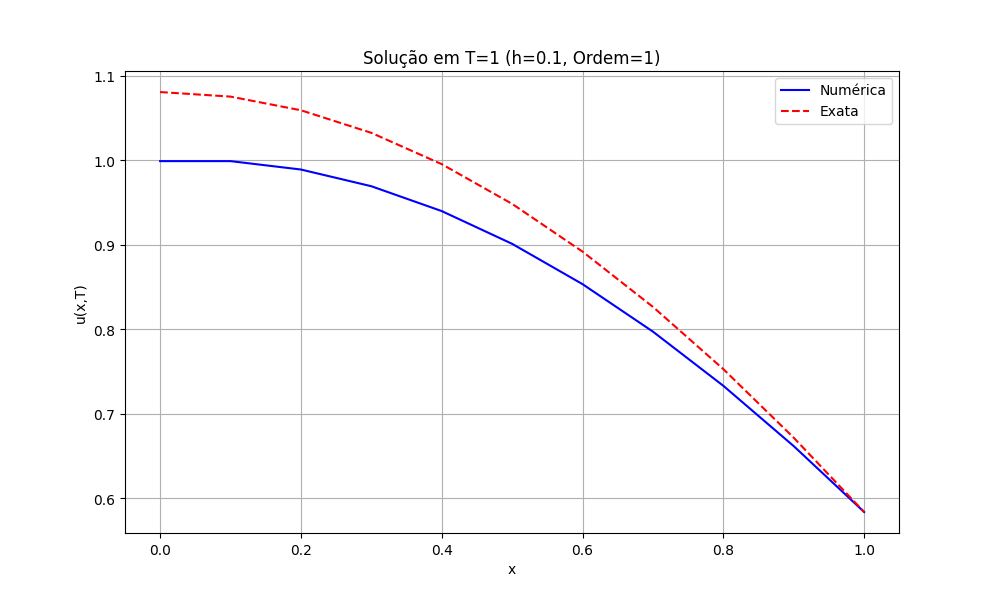
\includegraphics[width=\textwidth]{img/ex0101.png}
     \caption{Solução com $h=0.1$}
     \label{fig:ex1_1}
 \end{subfigure}
 \begin{subfigure}{0.35\textwidth}
     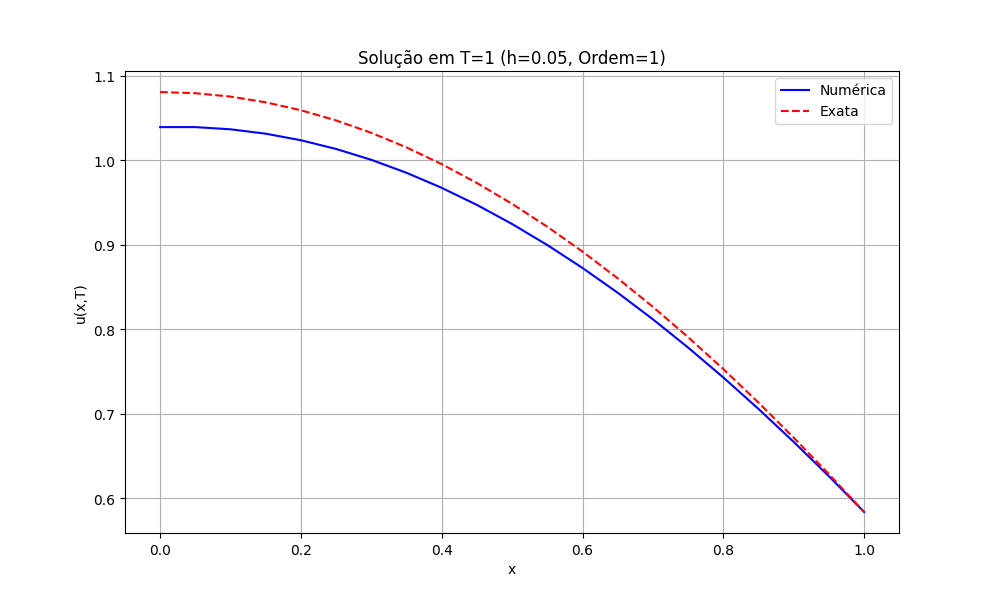
\includegraphics[width=\textwidth]{img/ex0102.png}
     \caption{Solução com $h=0.05$}
     \label{fig:ex1_2}
 \end{subfigure}
 \begin{subfigure}{0.35\textwidth}
     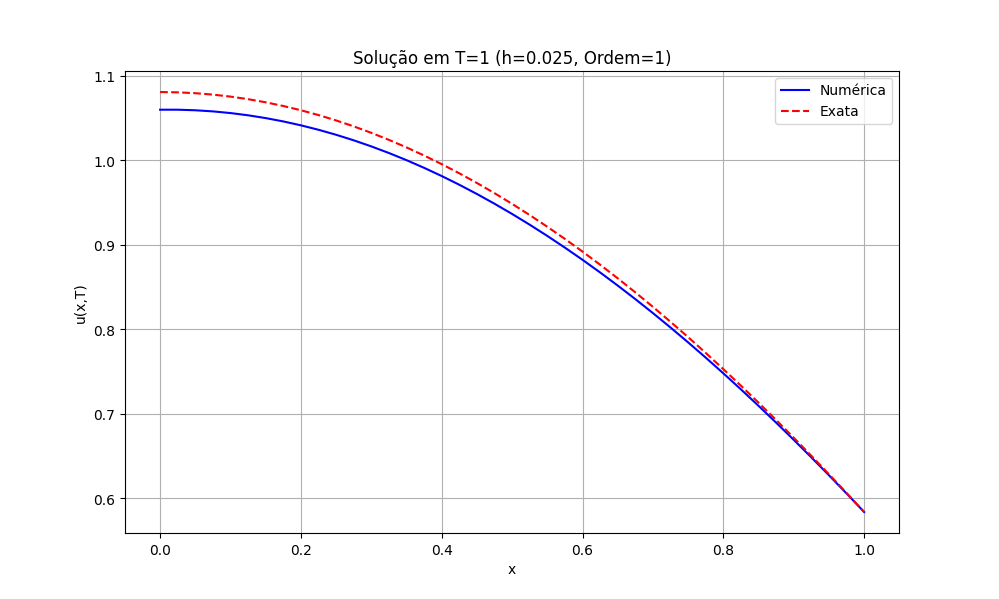
\includegraphics[width=\textwidth]{img/ex0103.png}
     \caption{Solução com $h=0.025$}
     \label{fig:ex1_3}
 \end{subfigure}
 \caption{Soluções numéricas com aproximação de primeira ordem}
 \label{fig:ex1_ord1}
\end{figure}

\begin{figure}[H]
 \centering
 \begin{subfigure}{0.35\textwidth}
     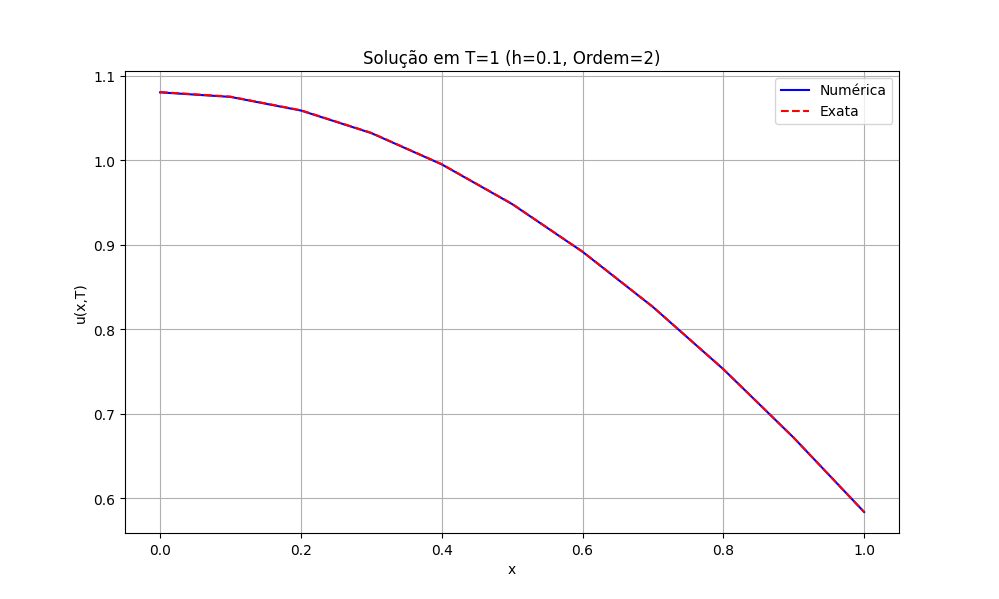
\includegraphics[width=\textwidth]{img/ex0104.png}
     \caption{Solução com $h=0.1$}
     \label{fig:ex1_4}
 \end{subfigure}
 \begin{subfigure}{0.35\textwidth}
     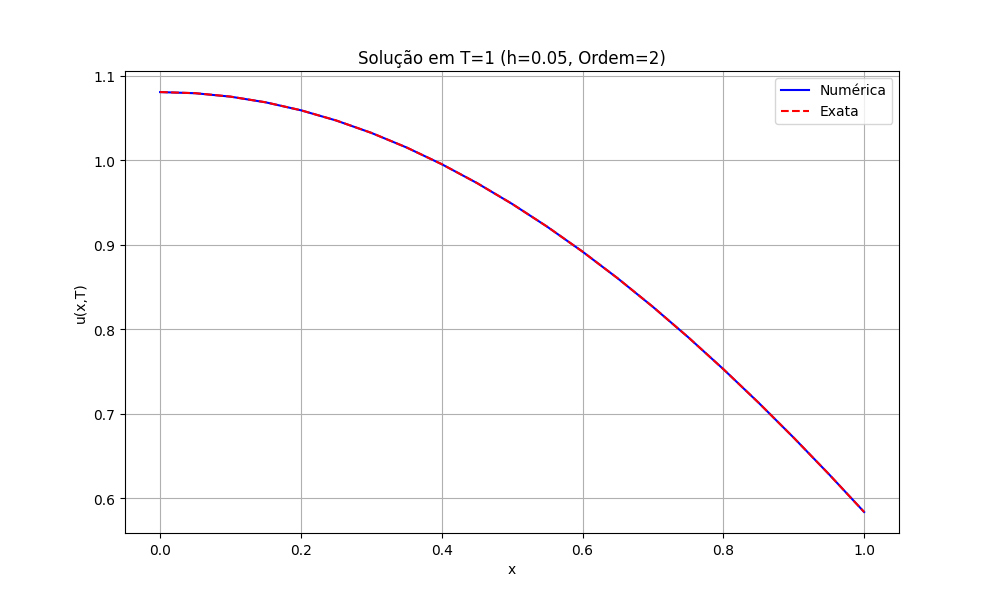
\includegraphics[width=\textwidth]{img/ex0105.png}
     \caption{Solução com $h=0.05$}
     \label{fig:ex1_5}
 \end{subfigure}
 \begin{subfigure}{0.35\textwidth}
     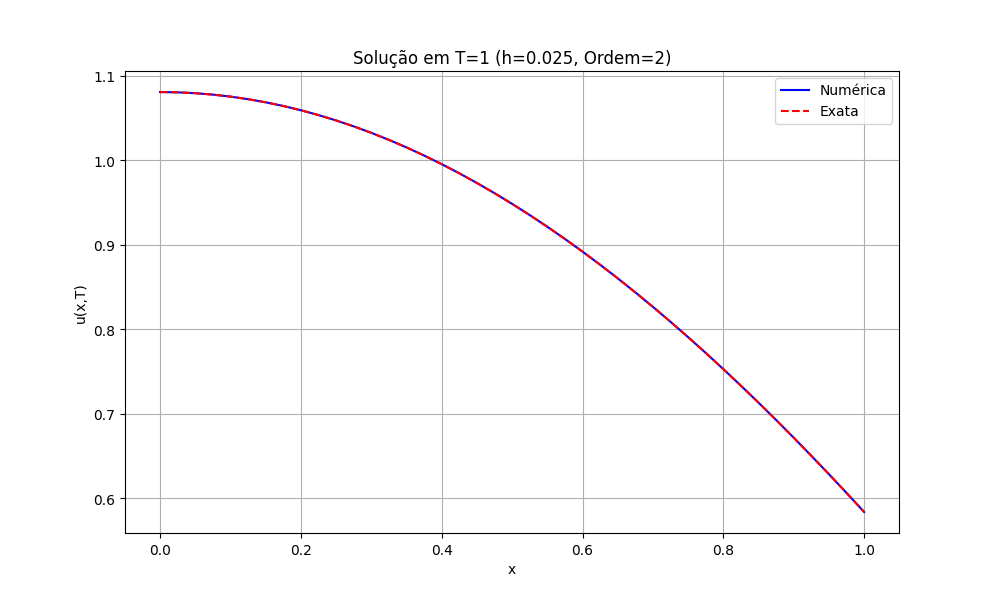
\includegraphics[width=\textwidth]{img/ex0106.png}
     \caption{Solução com $h=0.025$}
     \label{fig:ex1_6}
 \end{subfigure}
 \caption{Soluções numéricas com aproximação de segunda ordem}
 \label{fig:ex1_ord2}
\end{figure}

\begin{table}[H]
   \centering
   \caption{Erro máximo para diferentes valores de $h$ e ordens da condição de Neumann}
   \label{tab:erro_neumann}
   \renewcommand{\arraystretch}{1.25}
   \setlength{\tabcolsep}{12pt}
   \begin{tabular}{|c|c|c|}
       \hline
       \textbf{$h$} & \textbf{Ordem 1} & \textbf{Ordem 2} \\ \hline
       1/10 & 8.171035e-02 & 3.937531e-04 \\ \hline
       1/20 & 4.148152e-02 & 5.096550e-05 \\ \hline
       1/40 & 2.089094e-02 & 6.474309e-06 \\ \hline
   \end{tabular}
\end{table}

\subsection{Exemplo 02}

\begin{figure}[H]
 \centering
 \begin{subfigure}{0.35\textwidth}
     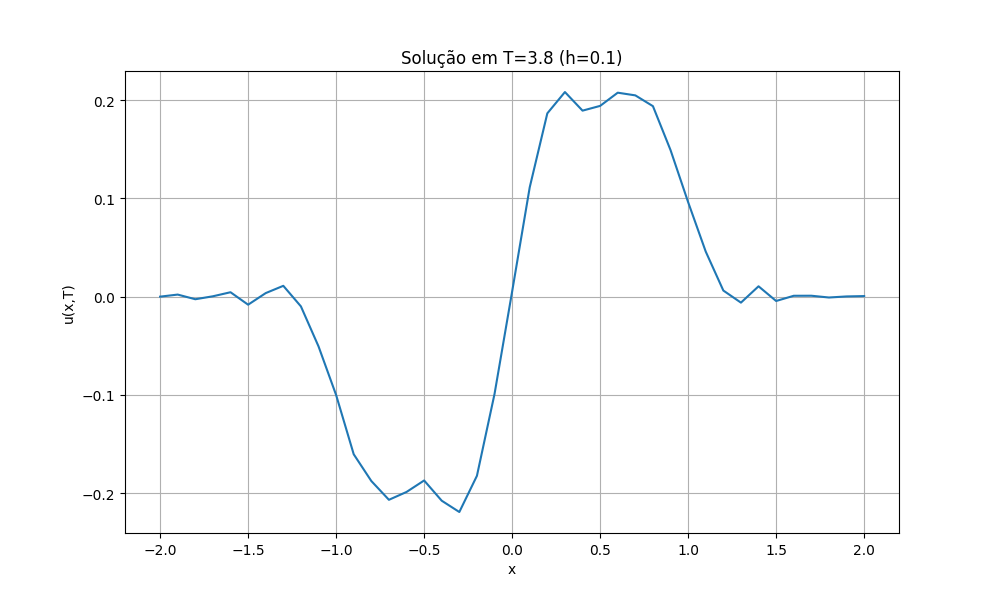
\includegraphics[width=\textwidth]{img/ex0201.png}
     \caption{Solução com $h=0.1$}
     \label{fig:ex2_1}
 \end{subfigure}
 \begin{subfigure}{0.35\textwidth}
     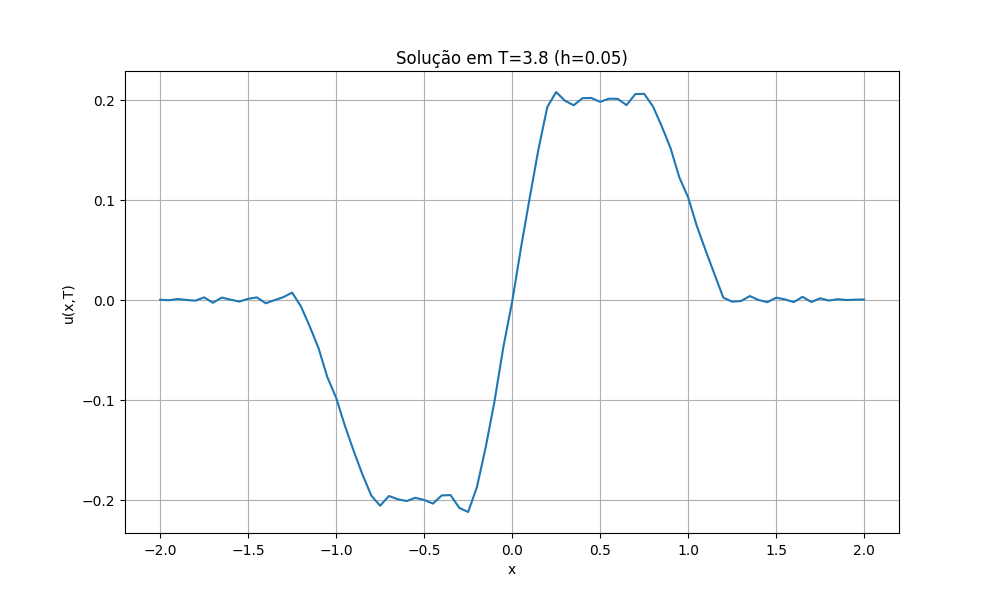
\includegraphics[width=\textwidth]{img/ex0202.png}
     \caption{Solução com $h=0.05$}
     \label{fig:ex2_2}
 \end{subfigure}
 \begin{subfigure}{0.35\textwidth}
     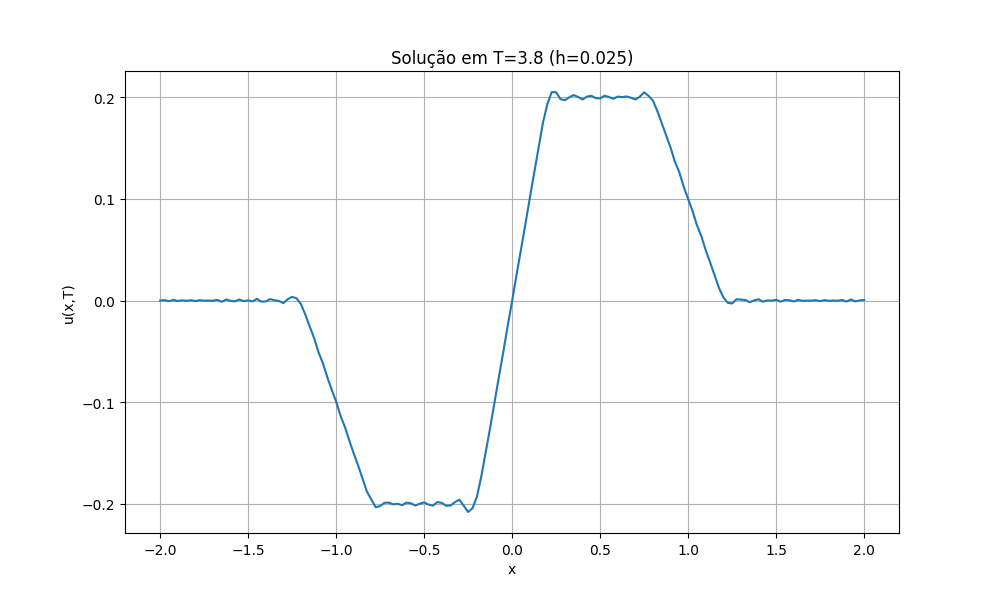
\includegraphics[width=\textwidth]{img/ex0203.png}
     \caption{Solução com $h=0.025$}
     \label{fig:ex2_3}
 \end{subfigure}
 \begin{subfigure}{0.35\textwidth}
     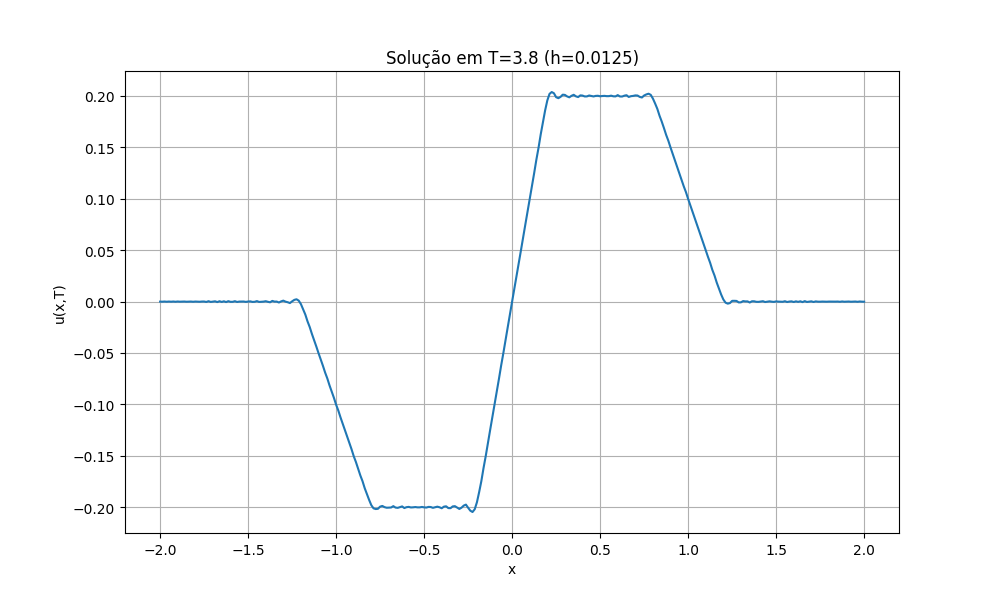
\includegraphics[width=\textwidth]{img/ex0204.png}
     \caption{Solução com $h=0.0125$}
     \label{fig:ex2_4}
 \end{subfigure}
 \caption{Convergência da solução numérica em $T=3.8$ para diferentes valores de $h$}
 \label{fig:ex2_conv}
\end{figure}

\begin{table}[H]
   \centering
   \caption{Análise do erro de simetria da solução em T=3.8}
   \label{tab:erro_simetria}
   \renewcommand{\arraystretch}{1.25}
   \setlength{\tabcolsep}{12pt}
   \begin{tabular}{|c|c|}
       \hline
       \textbf{$h$} & \textbf{Erro de simetria} \\ \hline
       0.100000 & 3.624836e-04 \\ \hline
       0.050000 & 1.345851e-04 \\ \hline
       0.025000 & 3.223981e-04 \\ \hline
       0.012500 & 5.543150e-05 \\ \hline
   \end{tabular}
\end{table}

\subsection{Exemplo 03}

\begin{figure}[H]
 \centering
 \begin{subfigure}{0.35\textwidth}
     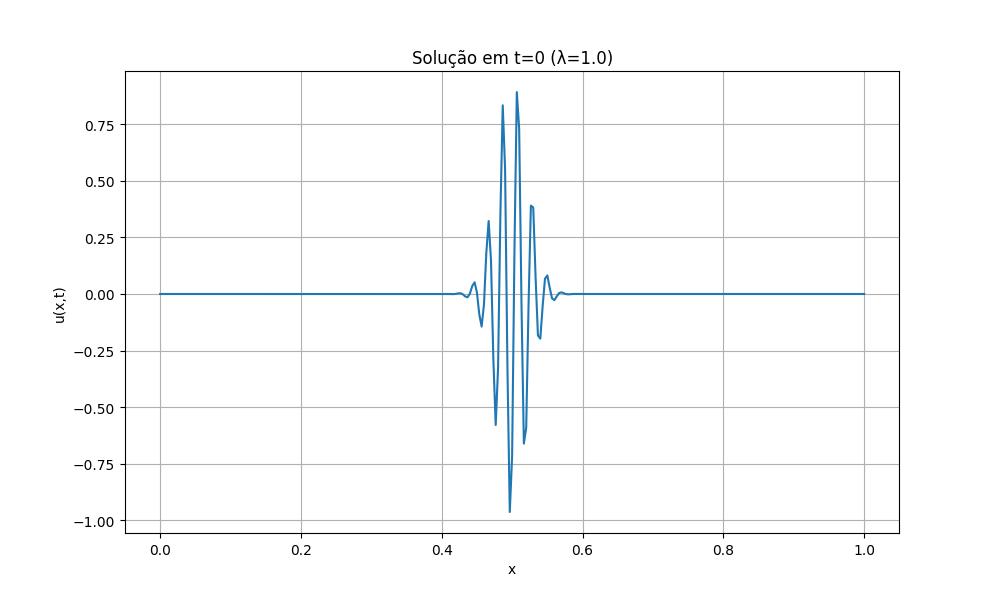
\includegraphics[width=\textwidth]{img/ex0301.png}
     \caption{Pulso inicial em $t=0$}
     \label{fig:ex3_1}
 \end{subfigure}
 \begin{subfigure}{0.35\textwidth}
     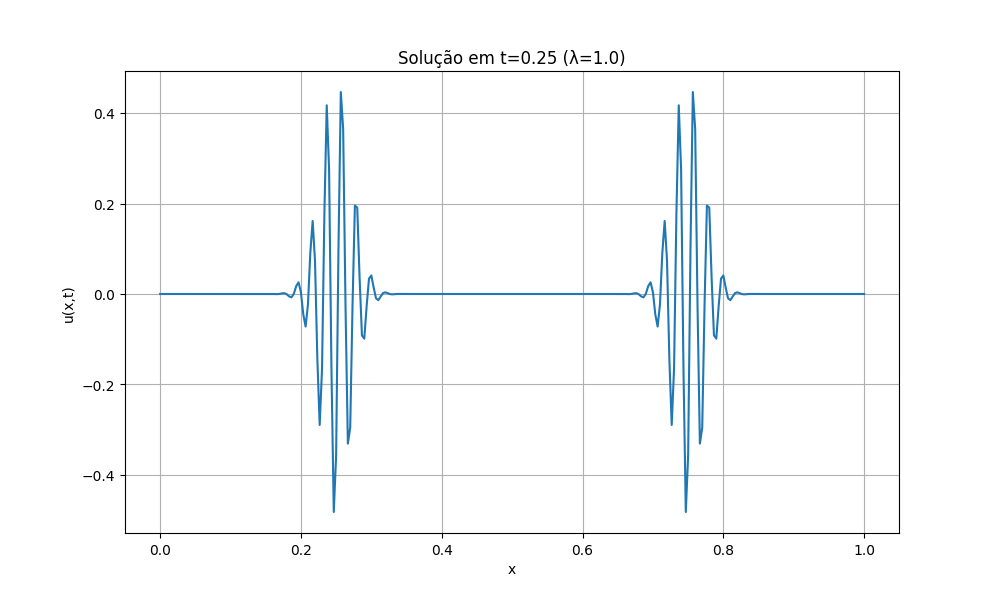
\includegraphics[width=\textwidth]{img/ex0302.png}
     \caption{Separação dos pulsos em $t=0.25$}
     \label{fig:ex3_2}
 \end{subfigure}
 \begin{subfigure}{0.35\textwidth}
     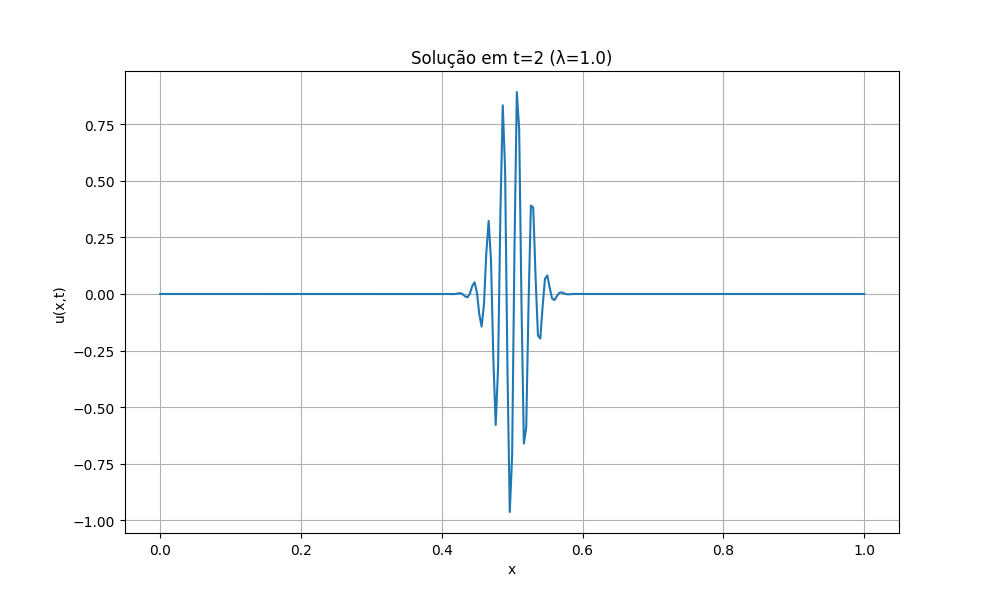
\includegraphics[width=\textwidth]{img/ex0303.png}
     \caption{Solução em $t=2$}
     \label{fig:ex3_3}
 \end{subfigure}
 \begin{subfigure}{0.35\textwidth}
     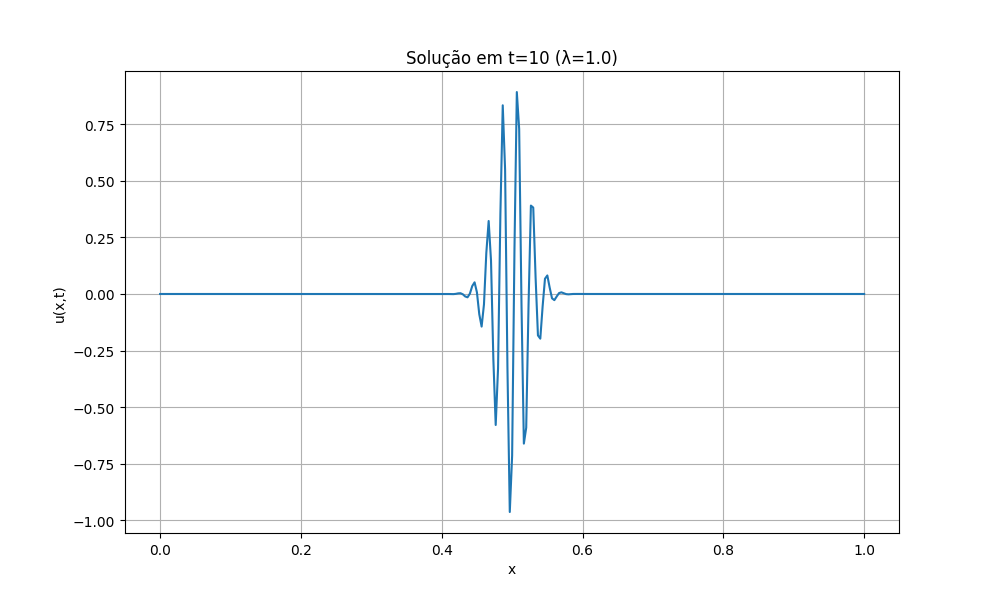
\includegraphics[width=\textwidth]{img/ex0304.png}
     \caption{Solução em $t=10$}
     \label{fig:ex3_4}
 \end{subfigure}
 \caption{Solução numérica com $\lambda=1.0$ e $h=1/300$}
 \label{fig:ex3_lambda1}
\end{figure}

\begin{figure}[H]
 \centering
 \begin{subfigure}{0.35\textwidth}
     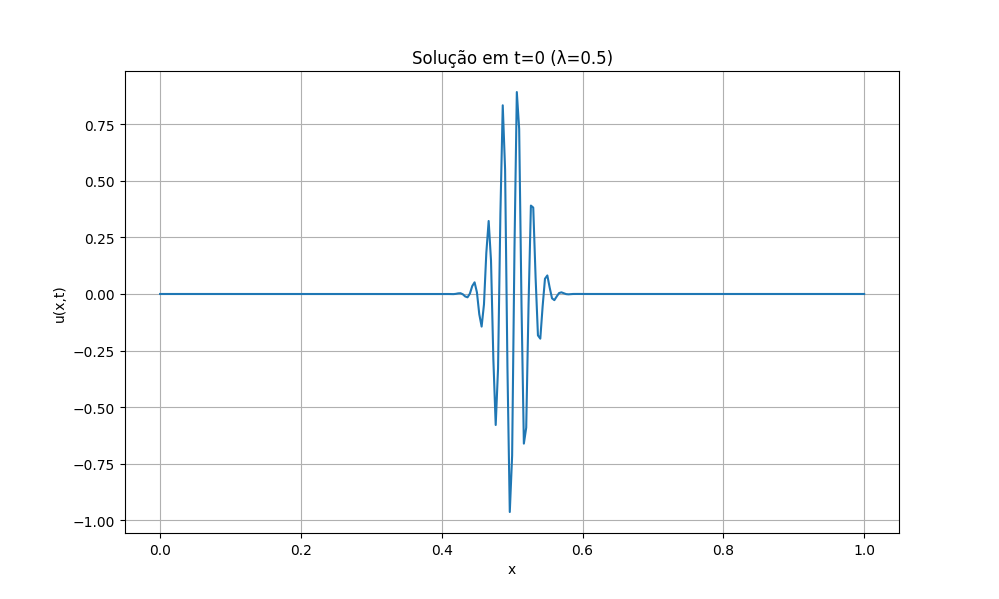
\includegraphics[width=\textwidth]{img/ex0305.png}
     \caption{Pulso inicial em $t=0$}
     \label{fig:ex3_5}
 \end{subfigure}
 \begin{subfigure}{0.35\textwidth}
     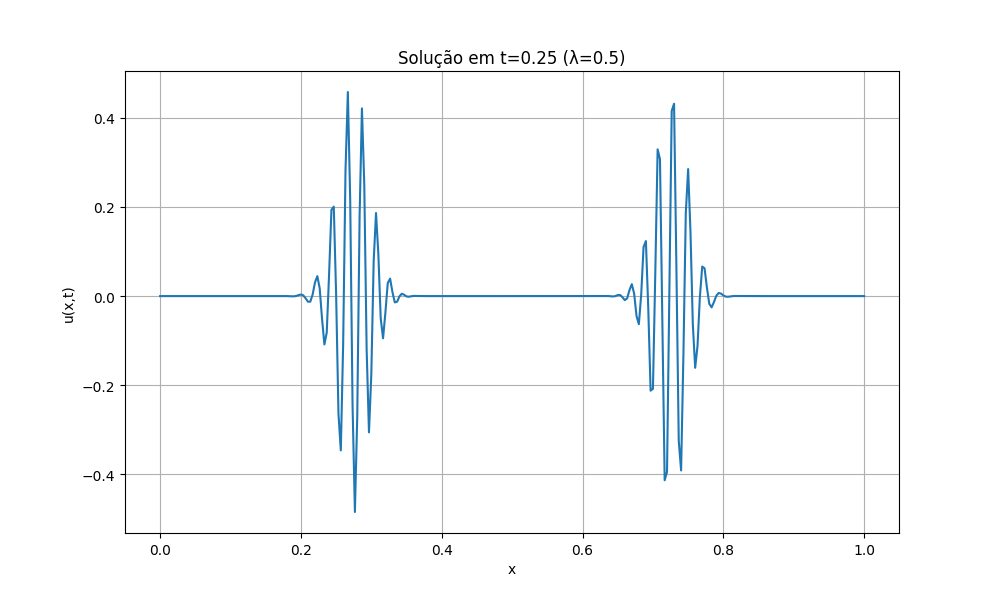
\includegraphics[width=\textwidth]{img/ex0306.png}
     \caption{Separação dos pulsos em $t=0.25$}
     \label{fig:ex3_6}
 \end{subfigure}
 \begin{subfigure}{0.35\textwidth}
     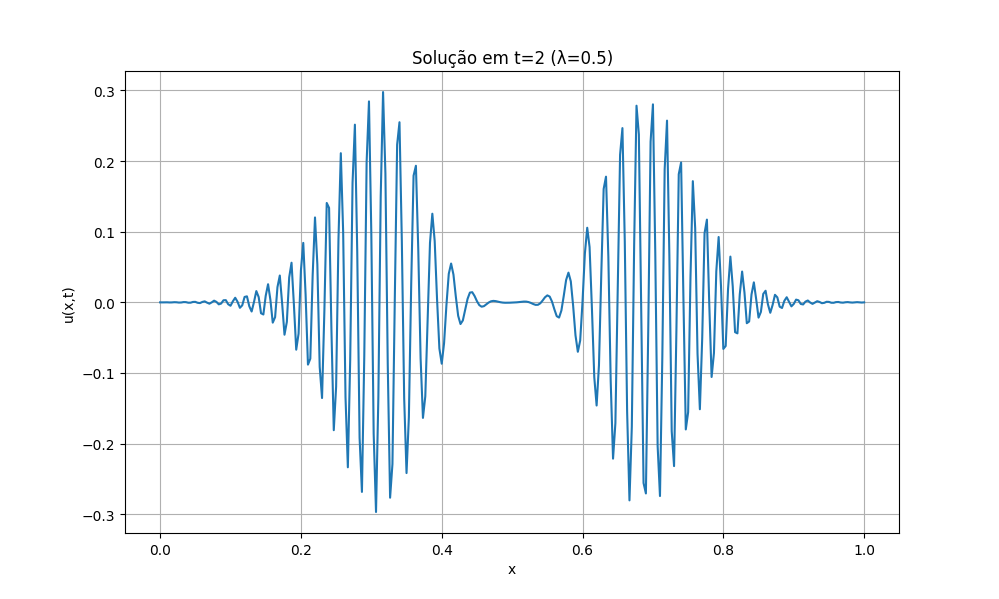
\includegraphics[width=\textwidth]{img/ex0307.png}
     \caption{Solução em $t=2$}
     \label{fig:ex3_7}
 \end{subfigure}
 \begin{subfigure}{0.35\textwidth}
     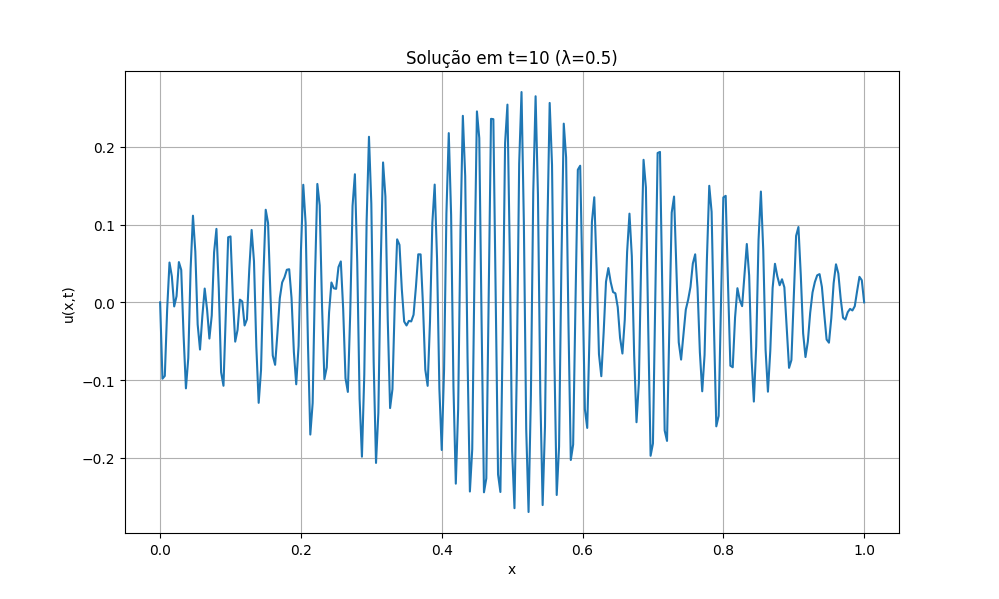
\includegraphics[width=\textwidth]{img/ex0308.png}
     \caption{Solução em $t=10$}
     \label{fig:ex3_8}
 \end{subfigure}
 \caption{Solução numérica com $\lambda=0.5$ e $h=1/300$}
 \label{fig:ex3_lambda05}
\end{figure}

\begin{table}[H]
   \centering
   \caption{Erro em relação à condição inicial para diferentes valores de $\lambda$}
   \label{tab:erro_lambda}
   \renewcommand{\arraystretch}{1.25}
   \setlength{\tabcolsep}{12pt}
   \begin{tabular}{|c|c|c|}
       \hline
       \textbf{$\lambda$} & \textbf{Erro em t=2} & \textbf{Erro em t=10} \\ \hline
       1.0 & 1.221245e-15 & 3.719247e-15 \\ \hline
       0.5 & 9.634010e-01 & 1.026740e+00 \\ \hline
   \end{tabular}
\end{table}

\section{Conclusão}
\section{Referências}

\end{document}